\documentclass{beamer}
% Use DS9 global theme (includes pgfplots for visualization)
\usepackage{../../../shared/templates/ds9_theme}

% Title page configuration
\title[1D Kinematics Review]{PHYS12 CH:1.1-1.4, 2.1-2.8}
\subtitle{Progression from Physics 11 to Physics 12: Advanced Kinematics}
\author[Mr. Gullo]{Mr. Gullo}
\date[Aug 28, 2025]{August 28, 2025}

\begin{document}
\frame{\titlepage}

\section{Introduction and Objectives}

\begin{frame}
\frametitle{Learning Objectives}
\framesubtitle{Reviewing the Fundamentals of Motion}
After this lesson, you will be able to:
\begin{itemize}
    \item Define position, displacement, distance, velocity, speed, and acceleration.
    \item Differentiate between vector and scalar quantities.
    \item Analyze one-dimensional motion under constant acceleration.
    \item Apply the kinematic equations to solve problems involving motion.
    \item Interpret position-time and velocity-time graphs to describe motion.
    \item Describe the motion of objects in free-fall.
\end{itemize}
\end{frame}

\begin{frame}
\frametitle{Physics 11 to Physics 12 Progression}
\framesubtitle{Building on Your Foundation}
\begin{itemize}
    \item \alert{Physics 11 Foundation}: Basic kinematic concepts, graphical analysis, and problem-solving methods
    \pause
    \item \alert{Physics 12 Enhancement}: More complex applications, vector analysis, and real-world scenarios
    \pause
    \item \alert{Key Progression Areas}:
    \begin{itemize}
        \item Multi-dimensional motion analysis
        \item Vector decomposition and composition
        \item Advanced problem-solving strategies
        \item Real-world applications and limitations
    \end{itemize}
\end{itemize}
\end{frame}

\section{Key Concepts}

\begin{frame}
\frametitle{Key Concepts}
\framesubtitle{Position, Displacement, and Distance}
\begin{description}
    \item[Position ($x$)] The location of an object at a particular time. It is a vector quantity.
    \pause
    \item[Displacement ($\Delta x$)] The change in an object's position. It is a vector pointing from the initial position ($x_0$) to the final position ($x_f$).
    \begin{center}
        $\Delta x = x_f - x_0$
    \end{center}
    \pause
    \item[Distance Traveled] The total length of the path traveled between two positions. It is a scalar quantity and is always positive.
\end{description}
\end{frame}

\begin{frame}
\frametitle{Concept Visualization}
\framesubtitle{Context: Displacement vs. Distance}
Imagine walking from your home to school.
\begin{itemize}
    \item The winding path you take along sidewalks represents the \alert{distance traveled}.
    \item A straight line drawn directly from your home to the school represents your \alert{displacement}.
\end{itemize}
\vspace{1em}
These two values are often different. Displacement only cares about the start and end points, not the path taken.
\end{frame}

\begin{frame}
\frametitle{Concept Visualization}
\framesubtitle{Displacement vs. Distance Traveled}
\begin{figure}
    \centering
    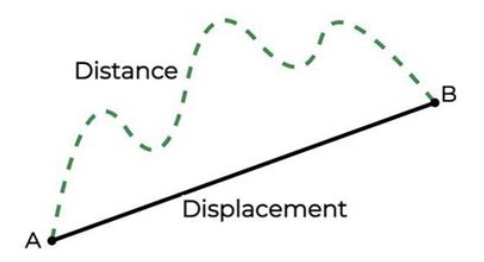
\includegraphics[width=0.7\linewidth]{phys12-mechanics-distance-displacement-diagram.png}
    \caption{Displacement is the shortest path, while distance is the actual path taken.}
\end{figure}
\end{frame}

\begin{frame}
\frametitle{Key Concepts}
\framesubtitle{Scalars vs. Vectors}
In physics, we use two types of quantities to describe the world:
\begin{columns}[T]
    \begin{column}{0.5\textwidth}
        \alert{Scalar}
        \begin{itemize}
            \item A quantity described by \textbf{magnitude} (a numerical value) only.
            \item Examples:
            \begin{itemize}
                \item Distance (5 m)
                \item Speed (10 m/s)
                \item Time (15 s)
                \item Mass (2 kg)
            \end{itemize}
        \end{itemize}
    \end{column}
    \begin{column}{0.5\textwidth}
        \alert{Vector}
        \begin{itemize}
            \item A quantity described by both \textbf{magnitude and direction}.
            \item Examples:
            \begin{itemize}
                \item Displacement (5 m, East)
                \item Velocity (10 m/s, North)
                \item Acceleration (9.8 m/s$^2$, Down)
                \item Force (20 N, Up)
            \end{itemize}
        \end{itemize}
    \end{column}
\end{columns}
\end{frame}

\begin{frame}
\frametitle{Key Concepts}
\framesubtitle{Velocity, Speed, and Acceleration}
\begin{description}
    \item[Average Speed] The total distance traveled divided by the elapsed time. A scalar.
    \pause
    \item[Average Velocity ($\bar{v}$)] Displacement divided by elapsed time. A vector.
    \[ \bar{v} = \frac{\Delta x}{\Delta t} = \frac{x_f - x_0}{t_f - t_0} \]
    \pause
    \item[Acceleration ($a$)] The rate at which velocity changes. A vector.
    \[ \bar{a} = \frac{\Delta v}{\Delta t} = \frac{v_f - v_0}{t_f - t_0} \]
    \textit{Deceleration} is simply acceleration in the direction opposite to the velocity.
\end{description}
\end{frame}

\begin{frame}
\frametitle{Key Concepts}
\framesubtitle{Free Fall}
\begin{itemize}
    \item An object in \alert{free-fall} is one that is moving under the influence of gravity alone (air resistance is considered negligible).
    \pause
    \item On Earth, all free-falling objects experience a constant downward acceleration, known as the \alert{acceleration due to gravity ($g$)}.
    \begin{center}
        $g = 9.80 \, \text{m/s}^2$
    \end{center}
    \pause
    \item The sign of acceleration depends on your chosen coordinate system. Conventionally, "up" is positive, which makes acceleration $a = -g = -9.80 \, \text{m/s}^2$.
\end{itemize}
\end{frame}

\section{The Kinematic Equations}

\begin{frame}
\frametitle{Essential Equations}
\framesubtitle{For Motion with Constant Acceleration}
These equations are the foundation for solving problems in 1D kinematics. They are only valid when acceleration \textit{a} is constant.
\begin{align*}
    v &= v_0 + at \\
    \Delta x &= v_0 t + \frac{1}{2}at^2 \\
    v^2 &= v_0^2 + 2a\Delta x \\
    \Delta x &= \frac{v_0 + v}{2} t
\end{align*}
\vspace{1em}
\begin{columns}[T]
    \begin{column}{0.5\textwidth}
        \textbf{Variables}
        \begin{itemize}
            \item $\Delta x$: displacement (m)
            \item $t$: elapsed time (s)
            \item $v_0$: initial velocity (m/s)
        \end{itemize}
    \end{column}
    \begin{column}{0.5\textwidth}
        \begin{itemize}
            \item $v$: final velocity (m/s)
            \item $a$: constant acceleration (m/s$^2$)
        \end{itemize}
    \end{column}
\end{columns}
\end{frame}

\section{Graphical Analysis}

\begin{frame}
\frametitle{Graphical Analysis of Motion}
\framesubtitle{Context: Position vs. Time Graph}
A graph of an object's position ($x$) as a function of time ($t$) provides a wealth of information about its motion.
\begin{itemize}
    \item The \alert{slope} of the line reveals the object's velocity.
    \item A straight line means constant velocity.
    \item A curved line means the velocity is changing (i.e., there is acceleration).
\end{itemize}
\vspace{1em}
On the next slide, we will visualize the difference between \alert{average velocity} (slope between two points) and \alert{instantaneous velocity} (slope at a single point).
\end{frame}

\begin{frame}
\frametitle{Graphical Analysis of Motion}
\framesubtitle{Visualization: Position vs. Time}
\begin{figure}
\begin{tikzpicture}
\begin{axis}[
    width=\textwidth,
    height=0.75\textheight,
    axis lines=left,
    xlabel={Time, $t$ (s)},
    ylabel={Position, $x$ (m)},
    xmin=0, xmax=5,
    ymin=0, ymax=14,
    xtick={0,1,2,3,4,5},
    ytick={0,2,4,6,8,10,12,14},
    legend pos=north west,
    label style={font=\large},
    tick label style={font=\small},
]
% Main curve: x = 0.5*t^2 + t
\addplot[ds9blue, thick, domain=0:4.5, samples=100, line width=1.5pt] {0.5*x^2 + x} node[right, pos=0.9] {$x(t)$};

% Secant line for average velocity between t=1 and t=4
\addplot[ds9gold, dashed, domain=1:4, line width=1.5pt] {2.5*x - 1};
\node[ds9gold] at (axis cs:3, 8) [above] {Avg. Velocity};
\fill[black] (axis cs:1, 1.5) circle (2pt);
\fill[black] (axis cs:4, 12) circle (2pt);

% Tangent line for instantaneous velocity at t=2
\addplot[ds9red, dotted, domain=0.5:3.5, line width=1.5pt] {3*x - 2};
\node[ds9red] at (axis cs:1.5, 1) [below] {Inst. Velocity};
\fill[black] (axis cs:2, 4) circle (2pt);

\end{axis}
\end{tikzpicture}
\end{figure}
\end{frame}

\begin{frame}
\frametitle{Graphical Analysis of Motion}
\framesubtitle{Context: Velocity vs. Time Graph}
A graph of velocity ($v$) versus time ($t$) also tells a detailed story.
\begin{itemize}
    \item The \alert{slope} of the line is the object's \textbf{acceleration}.
    \item The \alert{area under the curve} is the object's \textbf{displacement} ($\Delta x$).
\end{itemize}
\vspace{1em}
Next, we will see these two concepts illustrated for an object with constant positive acceleration.
\end{frame}

\begin{frame}
\frametitle{Graphical Analysis of Motion}
\framesubtitle{Visualization: Velocity vs. Time}
\begin{figure}
\begin{tikzpicture}
\begin{axis}[
    width=\textwidth,
    height=0.75\textheight,
    axis lines=left,
    xlabel={Time, $t$ (s)},
    ylabel={Velocity, $v$ (m/s)},
    xmin=0, xmax=5,
    ymin=0, ymax=12,
    xtick={0,1,2,3,4,5},
    ytick={0,2,4,6,8,10,12},
    legend pos=north west,
    label style={font=\large},
    tick label style={font=\small},
]
% Velocity line: v = 2*t + 1
\addplot[ds9blue, thick, domain=0:5, samples=2, line width=1.5pt] {2*x + 1} node[right, pos=0.8, anchor=south west] {$v(t)$};

% Annotate slope
\draw[ds9red, line width=1pt, <->] (axis cs:4.2, 5) -- (axis cs:4.2, 7) node[midway, right] {$\Delta v$};
\draw[ds9red, line width=1pt, <->] (axis cs:2, 5) -- (axis cs:3, 5) node[midway, below] {$\Delta t$};
\node[ds9red, align=center] at (axis cs:1.5, 8) {Slope = $a$};

% Shade area for displacement
\addplot[ds9gold!30, fill=ds9gold!30] coordinates {(0,1) (4,9) (4,0) (0,0)};
\node[black] at (axis cs:2, 2.5) {Area = $\Delta x$};

\end{axis}
\end{tikzpicture}
\end{figure}
\end{frame}

\section{Problem Solving Practice}

\begin{frame}
\frametitle{Problem Solving}
\framesubtitle{The GUESS Method}
We will use a structured method to solve physics problems.
\begin{itemize}
    \item \textbf{G} - \alert{Givens}: List all known quantities from the problem, with variables and units. Define your coordinate system (e.g., up is positive).
    \item \textbf{U} - \alert{Unknown}: Identify what quantity you need to find.
    \item \textbf{E} - \alert{Equation}: Choose a kinematic equation that relates your givens and unknown.
    \item \textbf{S} - \alert{Substitute}: Plug your known values into the equation, including units.
    \item \textbf{S} - \alert{Solve}: Calculate the answer and make sure it has the correct units and significant figures.
\end{itemize}
\end{frame}

\begin{frame}
\frametitle{I Do: Freeway Acceleration - Problem Setup}
\framesubtitle{Problem based on Ch. 2, Problem 24}
\begin{block}{Problem}
A car enters a freeway, accelerating from rest at a rate of $2.40 \, \text{m/s}^2$ for $12.0 \, \text{s}$. How far does the car travel in this time?
\end{block}
\pause
\begin{columns}[T]
\column{0.48\textwidth}
\begin{G - Givens}
\begin{itemize}
\item Direction of motion: positive
\item $\vec{a} = +2.40 \, \text{m/s}^2$, $t = 12.0 \, \text{s}$
\item $\vec{v}_0 = 0 \, \text{m/s}$ (starts from rest)
\end{itemize}
\pause
\column{0.48\textwidth}
\textbf{U - Unknown}
\begin{itemize}
\item $\Delta \vec{x} = ?$ (displacement)
\end{itemize}
\end{columns}
\end{frame}

\begin{frame}
\frametitle{I Do: Freeway Acceleration - Equation Selection}
\begin{columns}[T]
\column{0.48\textwidth}
\textbf{G - Givens}
\begin{itemize}
\item Direction of motion: positive
\item $\vec{a} = +2.40 \, \text{m/s}^2$, $t = 12.0 \, \text{s}$
\item $\vec{v}_0 = 0 \, \text{m/s}$ (starts from rest)
\end{itemize}
\pause
\column{0.48\textwidth}
\textbf{U - Unknown}
\begin{itemize}
\item $\Delta \vec{x} = ?$ (displacement)
\end{itemize}
\end{columns}
\pause
\begin{columns}[T]
\column{0.48\textwidth}
\textbf{E - Equation}
\begin{itemize}
\item Select: $\Delta x = v_0 t + \frac{1}{2}at^2$
\item Already solved for displacement
\end{itemize}
\end{columns}
\end{frame}

\begin{frame}
\frametitle{I Do: Freeway Acceleration - Solution}
\textbf{S - Substitute}
\begin{itemize}
\item Plug values with units:
\[ \Delta x = (0 \, \text{m/s})(12.0 \, \text{s}) + \frac{1}{2}(2.40 \, \text{m/s}^2)(12.0 \, \text{s})^2 \]
\end{itemize}
\pause
\textbf{S - Solve}
\begin{itemize}
\item Calculate with unit analysis:
\[ \Delta x = 0 + \frac{1}{2}(2.40 \, \text{m/s}^2)(144 \, \text{s}^2) \]
\[ \Delta x = (1.20 \, \text{m/s}^2)(144 \, \text{s}^2) = 172.8 \, \text{m} \]
\item Apply sig figs: $\alert{173 \, \text{m}}$
\item \boxed{173 \, \text{m}}
\end{itemize}
\end{frame}

\begin{frame}
\frametitle{We Do: Dolphin's Jump}
\framesubtitle{Problem based on Ch. 2, Problem 45}
\begin{block}{Problem}
A dolphin in an aquatic show jumps straight up out of the water at a velocity of $13.0 \, \text{m/s}$. How high does it rise above the water?
\end{block}
\pause
\begin{columns}[T]
\column{0.48\textwidth}
\textbf{G - Givens}
\begin{itemize}
\item Upwards is positive
\item $\vec{v}_0 = +13.0 \, \text{m/s}$, $\vec{a} = -9.80 \, \text{m/s}^2$
\item At max height: $\vec{v} = 0 \, \text{m/s}$
\end{itemize}
\pause
\column{0.48\textwidth}
\textbf{U - Unknown}
\begin{itemize}
\item $\Delta \vec{y} = ?$ (height)
\end{itemize}
\end{columns}
\end{frame}

\begin{frame}
\begin{columns}[T]
\column{0.48\textwidth}
\textbf{G - Givens}
\begin{itemize}
\item Upwards is positive
\item $\vec{v}_0 = +13.0 \, \text{m/s}$, $\vec{a} = -9.80 \, \text{m/s}^2$
\item At max height: $\vec{v} = 0 \, \text{m/s}$
\end{itemize}
\pause
\column{0.48\textwidth}
\textbf{U - Unknown}
\begin{itemize}
\item $\Delta \vec{y} = ?$ (height)
\end{itemize}
\end{columns}
\pause
\begin{columns}[T]
\column{0.48\textwidth}
\textbf{E - Equation}
\begin{itemize}
\item Select: $v^2 = v_0^2 + 2a\Delta y$
\item Rearrange: $\Delta y = \frac{v^2 - v_0^2}{2a}$
\end{itemize}
\end{columns}
\end{frame}

\begin{frame}
\textbf{S - Substitute}
\begin{itemize}
    \item Plug values: $\Delta y = \frac{(0)^2 - (13.0)^2}{2(-9.80)}$
\end{itemize}
\pause
\textbf{S - Solve}
\begin{itemize}
    \item Calculate: $\Delta y = \frac{0 - 169}{-19.6} = \frac{-169}{-19.6}$
    \item $\Delta y = 8.62 \, \text{m}$
    \item \boxed{8.62 \, \text{m}}
\end{itemize}
\end{frame}

\begin{frame}
\frametitle{You Do: Swan's Takeoff}
\framesubtitle{Problem based on Ch. 2, Problem 31}
\begin{block}{Problem}
A swan on a lake accelerates from rest at an average rate of $0.350 \, \text{m/s}^2$ to take off. It must reach a velocity of $6.00 \, \text{m/s}$ to get airborne.
\end{block}
\begin{enumerate}
    \item How far does it travel before becoming airborne?
    \item How long does this take?
\end{enumerate}

\begin{block}{Your Turn}
    Use the GUESS method to solve this problem on your own.
    \begin{itemize}
        \item List your givens and what you need to find for each part.
        \item Choose the appropriate equation for each part.
        \item Solve for one unknown at a time.
    \end{itemize}
\end{block}

\pause

\begin{beamercolorbox}[rounded=true,shadow=true]{info}
\centering
\textbf{Solution Check:} Your final answers should be (a) $\approx 51.4$ m and (b) $\approx 17.1$ s.
\end{beamercolorbox}

\end{frame}


\section{Conclusion}

\begin{frame}
\frametitle{Reading Homework}
\framesubtitle{Foundational Physics Concepts}
Please review these foundational sections for our next class:

\begin{itemize}
    \item \textbf{Section 1.5}: Physical Quantities and Units
    \item \textbf{Section 1.6}: Vector Addition and Subtraction
    \item \textbf{Section 1.7}: Vector Components
    \item \textbf{Section 1.8}: Relative Velocity
\end{itemize}

\begin{beamercolorbox}[rounded=true,shadow=true]{info}
\centering
\textbf{Focus on:} Understanding vector operations and relative motion concepts. These will be essential for our upcoming 2D motion unit.
\end{beamercolorbox}
\end{frame}

\begin{frame}
\frametitle{Summary}
\framesubtitle{Key Takeaways from 1D Kinematics}
\begin{itemize}
    \item \textbf{Scalars vs. Vectors}: Distance and speed are scalars; displacement, velocity, and acceleration are vectors (direction matters!).
    \pause
    \item \textbf{Constant Acceleration}: The kinematic equations are powerful tools, but they only apply when acceleration is constant. Free-fall is a key example ($a = -g$).
    \pause
    \item \textbf{Graphical Analysis}: Graphs provide a visual understanding of motion.
    \begin{itemize}
        \item Slope of position-time graph $\rightarrow$ velocity
        \item Slope of velocity-time graph $\rightarrow$ acceleration
        \item Area under velocity-time graph $\rightarrow$ displacement
    \end{itemize}
    \pause
    \item \textbf{Problem Solving}: A structured approach like the GUESS method is crucial for success.
\end{itemize}
\end{frame}

\begin{frame}
\frametitle{Homework: Physics 11 Review}
\framesubtitle{Essential Preparation for Advanced Topics}

To ensure success in Physics 12, please review these fundamental concepts from Physics 11:

\begin{itemize}
    \item \textbf{Chapter 1 Review}: Units, measurements, and significant figures
    \item \textbf{Chapter 2 Review}: Kinematic equations and problem-solving methods
    \item \textbf{Graphical Analysis}: Position-time and velocity-time graphs
    \item \textbf{Vector Basics}: Adding and subtracting vectors graphically
\end{itemize}

\begin{beamercolorbox}[rounded=true,shadow=true]{info}
\centering
\textbf{Focus on:} Mastering the GUESS method and understanding the difference between scalars and vectors. These skills will be critical for our upcoming 2D motion unit.
\end{beamercolorbox}

\end{frame}

\end{document}